\subsection{Experimental Method Proposal}
To encourage further research in this direction, we provide a sample reproducible explainability experiment. This includes dataset selection, graph formation and pre-processing, anomaly detection selection, and a compatible explainer. We provide both assumptions and examples within the context of fraud detection, with recommendations for results validation and ethical considerations.

\subsubsection{Dataset Selection and Pre-processing}
Both synthetic and real datasets are advantageous when creating or evaluating explainability models. Results generated from synthetic injected datasets can benefit from ground truth and supervision, while real data remains necessary to generalize models for real-world scenarios and train models on hidden complexities unaccounted for in generated data. The following fraud examples fulfill these requirements and are time-varying:

\begin{itemize}
    \item \textit{Elliptic dataset}\cite{weber_anti-money_2019}: a real cryptocurrency transaction dataset published by Weber, Domeniconi et al. and maintained by Elliptic.co.
    \item  \textit{BankSim dataset}\cite{lopez-rojas_banksim_2014}: a synthetic bank transaction dataset created by Dr. Lopez-Rojas.
    \item \textit{PaySim dataset}\cite{lopez-rojas_applying_2016}: a synthetic merchant transaction dataset created by Dr. Lopez-Rojas.
    \item \textit{Ebay dataset}\cite{rao_xfraud_2021}: a real customer transaction dataset curated by xFraud and licensed from Ebay Inc.
\end{itemize}

The following steps will utilize elliptic dataset due to its real data, generous licensing, and temporal graph structure. Elliptic transaction dataset is a collection of Bitcoin transactions that have been mapped and labeled specifically for financial network analysis and forensics. Each graph snapshot contains information about individual Bitcoin transactions, including the transaction ID, timestamp, input and output addresses, and the amount of Bitcoin transferred. Of the 203,769 nodes and 234,355 edges, only 23\% are labeled as either legitimate or illicit based on known fraudulent involvement\cite{weber_anti-money_2019}. Unfortunately, this means that the underlying model we choose to explain can't be monitored for performance via its true positive rate or true negative rate (sensitivity and specificity).

The common graph formation approach for this dataset is to represent nodes as transactions, with edges representing the flow of Bitcoin between transactions:

\clearpage
\begin{figure}
    \centering 
    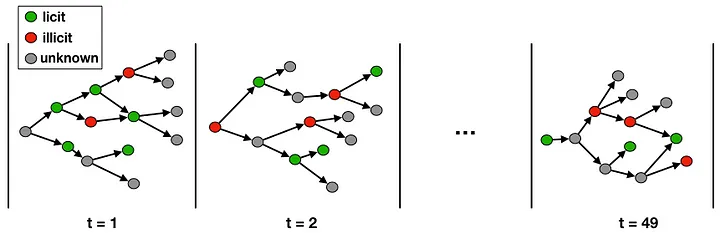
\includegraphics[width=\textwidth]{images/elliptic-sub-snap.png}
    \caption{Visualizatoin of elliptic subgraph structure over time \cite{bellei_elliptic_2019}. The Bitcoin blockchain is a directed acyclic graph (DAG). The Elliptic Data Set contains 49 connected components, from the earliest one at time step t = 1 to the later one at time step t = 49.}
    \label{fig:elliptic-sub-graphs}
\end{figure}

Transaction graphs that encode information in this format can be more difficult to analyze, as each node appears only once within a single time interval. This means that there is no node evolution between time intervals, making historical association difficult. Even though each time interval snapshot can be treated as a temporal graph, prior snapshots need to enhance classification using some other pattern or dimension because nodes will never reappear. This has interesting implications, as it suggests temporal models and explainers trained on traffic or brain prediction in other domains aren't suitable for transaction data in this arrangement. Based on our observation, most methods using node embeddings depend on node propagation history as an input and are also unsuitable. In fact, none of the models presented in Table \ref{table-3-full} are useful here due to the nature of the elliptic graphs. This example illustrates the importance of graph structure on model choice. EvolveGCN \ref{fig:EvolveGCN} shows how models can still effectively capture this temporal information using alternatives like LSTM or GRU. Trying to avoid this node embedding problem by mapping Bitcoin senders and receivers to nodes would create its own set of constraints: all temporal information would need to be re-encoded as edge features, and less developed edge embedding solutions would need to be used.

\subsubsection{Anomaly Detection Model Selection}
When selecting a detection model, it is important to consider compatibility, performance, and support for established frameworks. Since Elliptic dataset encodes temporal information via time-step, we need to focus on temporal graph analysis models.

Some preliminary analyses process the formed elliptic graphs through the use of GCNs\cite{karthika_gcn_2021}\cite{yang_transfer_2020} and autoencoder\cite{soto_fraud_2021}, though an existing published implementation exists via EvolveGCN\cite{pareja_evolvegcn_2019}.

DyHGN\cite{rao_modelling_2022} is another possiblility, as it was designed to deal with dynamic heterogeneous fraudulent transactional graphs. DyHGN is a dynamic extension of xFraud\cite{rao_xfraud_2021}, but unlike xFraud DyHGN uses Shapley Values instead of a GNNexplainer to explain graph-features via ab enriched XGBoost technique. This way, DyHGN avoids the complexity of explaining a dynamic heterogeneous network while benefiting from increased accuracy.

EvolveGCN\cite{pareja_evolvegcn_2019} is a RNN-GCN, using an RNN (via LSTM or GRU) to evolve its GCN's weights. Unlike the more common GCN-RNN proposed by \cite{narayan_learning_2018} and \cite{xie_explaining_2022} that suffers from cold starts, an RNN-GCN is able to predict fully dynamic graphs like Elliptic data. The main advantage of this technique is that it allows static explainers to be used. Amara et al.\cite{amara_graphframex_2022} mentions the effectiveness of perturbation technique for fraud explanation, and a GNNExplainer or modified GNNExplainer as proposed by \cite{rao_xfraud_2021} could be adapted to show important node/edge features that influenced specific instance classifications.

When selecting a model for graph analysis, code availability and support for established frameworks can be just as important as  for contributing reproducible, novel outcomes. Plan your technical implementation of the model around the intention to integrate the model, explainer, and dataset into a project like PyG\cite{pyg_team_pyg_nodate} or \cite{liu_pygod-teampygod_2023}. A meta framework like \cite{dive_lab_dig_nodate} may also be helpful in standardizing your data preparation and explainer wrapper with other implementations being developed.

\subsubsection{Explainers Selection}
The output of your anomaly detection model will be in the form of vectors containing anomalous embeddings. This is one of two components taken as an input into explainers. The other component will be some form of interfacing parameter that introspects EvolveGCN's black box process. We recommend picking a compatible temporal explainer to adapt based on the following criteria, in order of importance:

\begin{itemize}
    \item Actively developed with code available
    \item Merged into existing frameworks
    \item Published or used in order scenarios
    \item Known authors
\end{itemize}

We would advise against implementing the original EvolveGCN source; the temporal snapshot version of Elliptic has been recently integrated into PyG, and it would be both more novel and more reproducible for others to implement your model and explainer in PyG.

\subsubsection{Evaluation and Validation Metrics}
Evaluation and validation help quantify and verify the results of their machine learning models and explainers. If ground truth is available, check the underlying model's proportion of anomalies to total observations; if graphs are highly sparse, there is a higher proportion of false positives\cite{zhang_trustworthy_2022}. Fidelity scores can be used to measure precision via recall or F1 scores, as appropriate. Perturbation can be used after-the-fact to perform a sensitivity analysis to check which inputs most heavily affect explainer attributions. This could also be a potential source of bias.

Additional cross-validation with or without bootstrapping can be used to identify potential under- or over-fitting. This is accomplished by partitioning an existing dataset into training and validation sets, iteratively testing random subsets to evaluate performance on new data. Cross-validating with bootstrapping would require resampling the dataset and generating new subsets to evaluate variability and stability via distribution\cite{kauermann_statistical_2021}.

\subsection{Future Directions}
Further development of interpretability in dynamic graphs: Interpretability is highly valuable as it reduces the need for a secondary explanation model. The ongoing effort lies in developing accurate machine learning models that are inherently interpretable. However, there is still progress to be made in the field of time-specific interpretability, in areas like snap attention which are still in early stages of development.

Merging parallel work on GCN data loaders, explainable models, and frameworks: Merge orphan anomaly detection models and associated explainers into a parent framework like PyG, PyGoD, or Dive into Graphs to create a more reproducible research environment for the community.

Systems for streaming heterogenous graph data, live timestep-aware explainers: Contribute directly to the PyG team in an effort to adapt and implement live temporal or dynamic graph streaming.

Cost-aware models: Finding the optimal balance between true positives (TP) and false positives (FP) presents a significant challenge. However, by assigning costs to TP and FP, it becomes feasible to identify the most financially advantageous model for companies.

Performing a systematic analysis of bank costs associated with false positives (overly sensitive) and false negatives (camouflaging) due to the implementation of a cost-aware detection model is crucial in financial systems. Surprisingly, there are only a limited number of papers that specifically focus on cost considerations for the bank or companies in this context. Therefore, developing a cost aware detection model is a potential avenue for future research.

Model-based explanation: Instance-based explanations have seen greater development compared to model-based explanations. This is primarily due to the challenge of comprehending a large and complex set of rules that arise when attempting to explain the entire model's decision for all nodes. However, in cases where the graph is small or when anomalies exhibit redundant patterns, model-based explanations can be beneficial.

For dynamic graphs, we propose exploring snap-based explanations, which can be particularly valuable when encountering frequently processing similar fraud data. Additionally, snapshot graphs tend to be smaller than static graphs since more snapshots need to be stored. This presents a potential application for model/snapshot-based explainers.